\chapter{Etat de l'art}
\section*{Introduction}
Dans ce chapitre, Nous analysons les principales pratiques et les outils les plus adaptés à notre projet. Nous commençons par introduire les concepts de DevOps, CI/CD, Cloud Computing et IaC. Après, nous mettons l'accent sur l’intégration du cloud dans notre solution DevOps et l'intégration de l'IaC dans notre solution cloud. En conclusion, nous effectuons une analyse comparative des outils tout en synthétisant nos choix optés.

\section{Approche DevOps}
L'approche DevOps \cite{crochetdamais2019} regroupe un ensemble de techniques qui met en relief l'automatisation des tâches entre l'équipe de développement de logiciels (Dev) et l'équipe d'exploitation informatique (Ops), comme le montre la figure \ref{fig:devops} \cite{kim2022}.
        \begin{figure}[H]
        \centering
        \frame{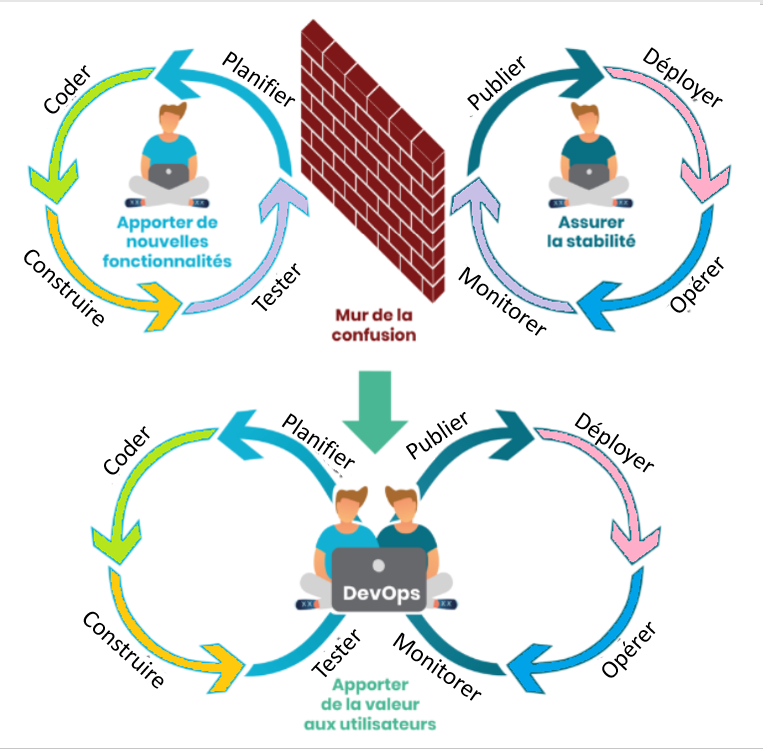
\includegraphics[width=16cm, height=12cm]{img/5.png}}
        \caption{Approche DevOps.}
        \label{fig:devops}
        \end{figure}
Les deux équipes alors se collaborent ensemble du début à la fin du cycle de vie des applications, depuis le développement et les tests, jusqu' au déploiement et à l'exploitation. Le but est d'accélérer la livraison des applications par rapport aux méthodes de développement traditionnelles. Cette collaboration améliore la réactivité de l'entreprise, la rendant plus compétitive et plus apte à satisfaire ses clients sur le marché.

\section{Intégration continue et déploiement continu CI/CD}

Le CI/CD est une technique clé dans l'approche DevOps, composée de deux pratiques fondamentales : l'intégration continue (CI) et la livraison et déploiement continus (CD).\\
L'intégration continue (CI) \cite{moronval2020} permet de fusionner fréquemment les modifications de code et déclenche un processus automatisé de construction et de test pour vérifier le bon fonctionnement de l'application. Cette pratique vise à identifier rapidement les conflits ou les erreurs dans le code, permettant ainsi de les résoudre de manière efficace et rapide. En cas de conflit entre le code actuel et le nouveau code ou en cas d'erreur dans le code, la CI intervient immédiatement pour résoudre le problème, minimisant ainsi les interruptions de développement. \\
La livraison continue va un pas plus loin en s'assurant que le code validé est toujours dans un état déployable. Alors que, Le déploiement continu (CD) \cite{crochetdamais2023}, complète l'intégration et la livraison continues. Il garantit que les modifications validées sont automatiquement déployées dans un environnement de production, tel que le cloud. Cette pratique permet de minimiser les risques associés aux déploiements manuels et de rendre les nouvelles fonctionnalités immédiatement disponibles aux utilisateurs.\\
Le déploiement continu assure une livraison fluide et ininterrompue des mises à jour, facilitant une réponse rapide aux retours des utilisateurs et aux besoins du marché. La figure \ref{fig:cid} \cite{veritis2024} indique les éléments de pipeline les plus courantes.
        \begin{figure}[H]
        \centering
        \frame{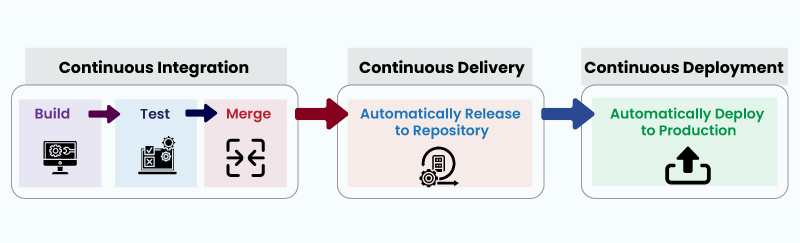
\includegraphics[width=16cm, height=6.5cm]{img/continuous-deployment.jpg}}
        \caption{Éléments de pipeline CI/CD.}
        \label{fig:cid}
        \end{figure}

\section{Conteneurisation et virtualisation cloud}
La virtualisation et la conteneurisation sont deux technologies utilisées lors de la phase de déploiement. Nous allons maintenant les introduire. La conteneurisation \cite{axopen2021docker} repose sur l'utilisation de logiciels tels que Docker, permettant de se passer d'un système d'exploitation distinct pour chaque conteneur. Ce concept est illustré par la figure \ref{fig:cont} \cite{strauss2020}. Dans ce contexte, toutes les dépendances de l'application sont regroupées dans un conteneur. Les ressources, telles que l'espace et la mémoire, ne sont pas fixées, mais allouées en fonction des besoins de l'application, éliminant ainsi la surcharge. Cette approche offre de meilleures performances en termes de rapidité et de légèreté. Nous l'utiliserons ensuite pour créer nos conteneurs Asterisk et MySQL.
\begin{figure}[H]
        \centering
        \frame{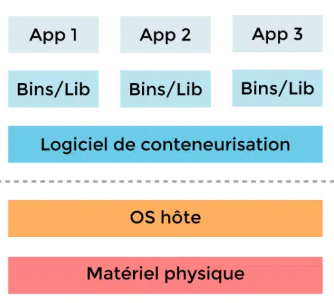
\includegraphics[width=7.5cm, height=5cm]{img/Conteneurisation.PNG}}
        \caption{Conteneurisation.}
        \label{fig:cont}
        \end{figure}
Cependant, la virtualisation \cite{samarakoon2023} repose sur un hyperviseur pour créer et exécuter plusieurs machines virtuelles sur un système hôte, comme le montre la figure \ref{fig:virtual} \cite{strauss2020}. Chaque machine virtuelle possède son propre système d'exploitation. 
\begin{figure}[H]
        \centering
        \frame{\includegraphics[width=7.5cm, height=6.5cm]{img/virtual.PNG}}
        \caption{Virtualisation.}
        \label{fig:virtual}
        \end{figure}
Cette approche peut surcharger la plate-forme hôte puisque des quantités fixes de mémoire et d'espace sont allouées à chaque machine virtuelle, ce qui peut entraîner un gaspillage significatif de ressources. D'où, nous décisions de passer à La virtualisation cloud qui présente plusieurs avantages significatifs en termes de flexibilité et de gestion des ressources. Les fournisseurs de Cloud Computing utilisent cette technologie pour optimiser l'utilisation des ressources physiques, créant ainsi des environnements isolés et sécurisés pour chaque utilisateur. Cela permet de provisionner, déployer et gérer facilement nos ressources tout en répondant aux besoins de l'entreprise et en maximisant l'efficacité opérationnelle.

\section{Cloud Computing}
Le Cloud Computing \cite{Plu2019} ou l'informatique en nuage présente un service qui fournit un ensemble de ressources informatiques accessibles via Internet. Il offre la possibilité de stocker et de gérer les données, les logiciels et les applications sur des serveurs. Nous pouvons le classer en trois types, selon le mode d'hébergement, comme indiqué dans la figure \ref{fig:cloud} \cite{syloe2018}.
        \begin{figure}[H]
        \centering
        \frame{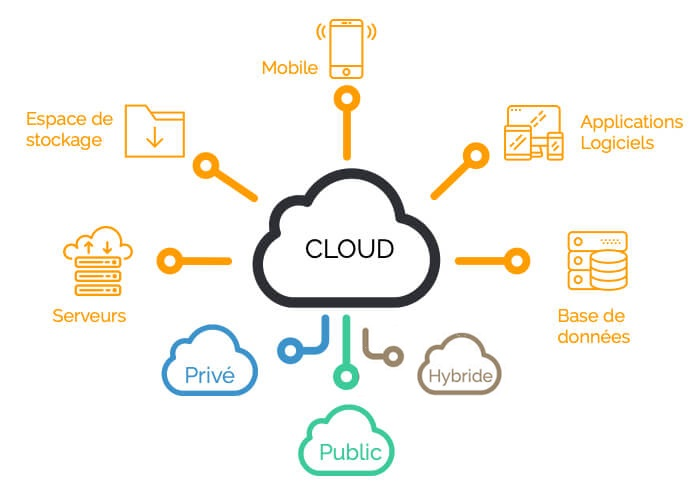
\includegraphics[width=16cm, height=9cm]{img/schema-cloud.jpg}}
        \caption{Types de Cloud Computing.}
        \label{fig:cloud}
        \end{figure}
\begin{itemize}
    \item \textbf{Cloud public} : il met à disposition des ressources publiques fournies par un fournisseur tiers. Il permet à de multiples utilisateurs d'accéder aux mêmes services et infrastructures via Internet. C'est une solution économique et évolutive, idéale pour les applications non sensibles aux données et nécessitant une évolutivité rapide.
    \item \textbf{Cloud privé} : il propose des services cloud propres à une entreprise, accessibles uniquement en interne, afin de garder la main sur l'infrastructure et répondre aux exigences strictes en matière de sécurité et de conformité.
    \item \textbf{Cloud hybride} : il s'agit d'une combinaison du cloud public et du cloud privé, où l'entreprise utilise ses propres ressources internes pour des tâches critiques tout en exploitant des ressources cloud publiques pour des opérations moins sensibles aux données. Cela offre une plus grande flexibilité et optimise les coûts en fonction des besoins spécifiques de l'organisation.
\end{itemize}
\section{Approche IaC}
L’infrastructure as code (IaC) sert à écrire un code qui automatise la création et la configuration de l'infrastructure informatique à travers des langages de codage descriptifs de haut niveau. Grâce à cette automatisation, l'équipe DevOps n’a plus besoin de configurer et de gérer manuellement les ressources chaque fois qu’ils développent, testent ou déploient une application logicielle.
Grâce à l'IaC, les environnements d'infrastructure, tels que les serveurs, les réseaux et les bases de données, peuvent être définis et gérés de manière cohérente et reproductible. Cela simplifie le processus de déploiement et garantit que l'infrastructure est toujours configurée de manière optimale et conforme aux besoins de l'application. Par exemple, en utilisant des outils comme Terraform, les équipes peuvent décrire leur infrastructure cible dans des fichiers de configuration. Ces fichiers sont ensuite exécutés pour déployer et mettre à jour automatiquement les ressources nécessaires, que ce soit dans des environnements locaux, dans le cloud ou dans des architectures hybrides. Cela permet de réduire les erreurs humaines, d'améliorer la sécurité et de simplifier la gestion globale des infrastructures informatiques.

\section{Intégration de Cloud Computing dans la solution DevOps}
L’objectif d’une solution DevOps est d’accélérer la mise en production des applications tout en présentant une meilleure qualité. Bien que DevOps soit une approche indépendante du cloud, ce dernier joue un rôle très important pour renforcer son efficacité. Il sert à simplifier la mise en place et la gestion de l’infrastructure nécessaire pour l’exécution d’une application. Grâce au cloud, les équipes DevOps peuvent facilement provisionner et configurer des environnements d'exécution, ce qui permet une intégration continue rapide et une livraison continue des applications. Cela conduit à une satisfaction accrue de l'utilisateur final, car les mises à jour et les nouvelles fonctionnalités sont déployées plus rapidement et de manière plus fiable. De plus, le cloud offre une solution économique pour le déploiement des applications, car il permet de réduire les coûts liés à l'achat et à la gestion d'infrastructures physiques. Les fournisseurs de cloud proposent également une gamme étendue d'outils et de services qui simplifient les opérations de développement et d'exploitation, comme le stockage de données, la gestion des identités, et les services de sécurité.

\section{Intégration de l'approche IaC dans le Cloud Computing}
Le cloud computing favorise l'approche Infrastructure as Code (IaC). Grâce à cette méthode, nous pouvons créer, modifier et supprimer nos ressources cloud en utilisant un code automatisé. Cela contribue à la rapidité et à la facilité de gestion de l'infrastructure cloud. En utilisant des outils comme Terraform, Ansible, ou CloudFormation, les équipes peuvent décrire leur infrastructure cible dans des fichiers de configuration. Ces fichiers sont ensuite exécutés pour déployer et mettre à jour automatiquement les ressources nécessaires dans le cloud. Cette automatisation permet de réduire les erreurs manuelles, d'améliorer la cohérence et de garantir que l'infrastructure est toujours configurée de manière optimale. De plus, l'IaC facilite la reproductibilité et la scalabilité des environnements cloud. Les configurations peuvent être répliquées facilement d'un environnement à un autre, par exemple, du développement à la production, assurant ainsi une uniformité et une conformité constantes.

\section{Etude comparative des outils}
Il existe différents outils sur le marché pour notre solution proposée, ce qui rend le choix difficile, d'où la nécessité d'une étude comparative pour faire le bon choix selon nos besoins.

\subsection{Outils de gestion des versions}
La gestion des versions \cite{axopen} enregistre les changements apportées au code source d'une application, facilitant la collaboration entre l'équipe et la récupération de versions spécifiques. Elle permet le travail sur plusieurs branches, la gestion des modifications, et la résolution des problèmes de fusion.
Cette étude sur la gestion des versions, illustrée dans le tableau \ref{tableau:comparatif3} \cite{strauss2018}, vise à consolider le choix de l'outil GitHub, déjà utilisé en interne, par rapport à ses concurrents GitLab et BitBucket.
\begin{table}[H]
\centering
\caption{Tableau comparatif des outils de gestion des versions GitHub, Gitlab et Bitbucket.}
\begin{longtable}{|p{3.5cm}|p{3.75cm}|p{3.75cm}|p{3.75cm}|}
\hline
\textbf{Critères de comparaison} & \textbf{GitHub Entreprise} & \textbf{GitLab Ultimate} & \textbf{Bitbucket Premium}\\
\hline
\textbf{Propriétaire} & Microsoft & GitLab Inc. & Atlassian \\
\hline
\textbf{Language} & Ruby & Ruby, Go, Vue.js & Python\\
\hline
\textbf{Open-source} & Non & Oui & Non \\
\hline
\textbf{Integrations} & Jira, Microsoft Teams, Slack, Microsoft Azure & Jira, Bugzilla, Custom Issue, Tracker & Jira, Trello, Bamboo, Opsgenie \\ 
\hline
\textbf{CI/CD en minutes par mois} &  50.000 &  50.000 & 3.500 \\
\hline
\textbf{Limite de stockage} & 50 GB  &  60\$ pour chaque ajout de 10 GB & 10 GB \\
\hline
\textbf{Coût d'un utilisateur par mois} & 21\$ & 99\$ & 6\$\\
\hline
\textbf{Communauté} & Robuste & Active & Limitée\\
\hline
\end{longtable}
\label{tableau:comparatif3}
\end{table}
GitHub est l'outil choisi, étant donné qu'il propose diverses fonctionnalités de gestion des versions. Il offre une grande variété d'intégrations avec des outils couramment utilisés. De plus, GitHub Actions fournit un temps d'exécution important pour les pipelines CI/CD, et des limites de stockage largement flexibles pour répondre à nos besoins. Il dispose également d'une communauté solide. En outre, il présente l'avantage d'être moins coûteux que GitLab et GitLab CI/CD.

\subsection{Outils de conteneurisation}
Docker et Podman sont les plus populaires outils de conteneurisation. Le tableau \ref{tableau:comparatif2} \cite{aleksic2022} permet de comparer ces deux outils afin de retenir l’outil qui satisfait au mieux les besoins de l’entreprise.
\begin{table}[H]
\centering
\caption{Tableau comparatif des outis de conteneurisation Docker et Podman.}
\begin{longtable}{|p{4.5cm}|p{5.5cm}|p{5.5cm}|}
\hline
\textbf{Critères de comparaison} & \textbf{Docker} & \textbf{Podman} \\
\hline
\textbf{Technologie de conteneur} & Utilise Docker Engine & Utilise le moteur Podman \\
\hline
\textbf{Architecture} & Utilise le démon Docker & Sans démon \\
\hline
\textbf{Privilèges de l'utilisateur} & Super utilisateur & Super utilisateur et utilisateur ordinaire \\
\hline
\textbf{Images} & Création d'images de conteneur & Utilise Buildah pour créer des images de conteneur \\ 
\hline
\textbf{Orchestration} & Docker Swarm, utilisable avec Kubernetes & Utilisable avec Kubernetes  \\ 
\hline
\textbf{Utilisation dans l'industrie} & Largement utilisé et bien documenté & Outil plus récent, moins utilisé, documentation moins abondante\\
\hline
\textbf{Système d'exploitation} & Linux, Windows, macOS & Linux, Windows (avec WSL), macOS\\
\hline
\end{longtable}
\label{tableau:comparatif2}
\end{table}

Après une analyse comparative, notre choix s'est porté sur Docker en raison de sa large adoption, de ses performances fiables grâce à Docker Engine, et de sa flexibilité. Il repose sur une architecture client-serveur avec un démon. Il bénéficie d'une documentation complète. De plus, cet outil propose Docker Swarm pour l'orchestration des conteneurs, et peut également être intégré avec Kubernetes. Le logiciel est aussi compatible avec plusieurs systèmes d'exploitation, présentant alors un choix solide pour notre équipe DevOps.

\subsection{Outils d'approvisionnement de l'infrastructure}
Grâce à des outils d'approvisionnement de l'infrastructure, nous n'avons pas besoin de créer nos ressources manuellement, il suffit d'exécuter le code de notre infrastructure qui effectue toute la configuration sur le cloud.
Le tableau \ref{tableau:terraform} \cite{Kadima2024} synthétise une série de critères de comparaison entre Terraform et Ansible permettant de trancher sur l’outil IaC qui satisfait au mieux les besoins de l’entreprise.
\begin{table}[H]
\centering
\caption{Tableau comparatif des outils de gestion et d’automatisation des configurations Terraform et Ansible.}
\begin{longtable}{|p{4.5cm}|p{5.25cm}|p{5.25cm}|}
\hline
\textbf{Critères de comparaison} & \textbf{Terraform} &\textbf{Ansible} \\ 
\hline
\textbf{Type} & Infrastructure as Code (IaC) & Configuration Management \\
\hline
\textbf{Architecture} & Sans agent & Sans agent \\
\hline
\textbf{Language} & HCL & YAML/Ansible Playbooks\\
\hline
\textbf{Syntaxe} & Déclarative & Impérative \\
\hline
\textbf{Installation} & Facile & Facile \\
\hline
\textbf{Support des clouds} & Multi-cloud & Multi-cloud \\
\hline
\textbf{Approche par défaut} & Approvisionnement et orchestration des infrastructures & Configuration et gestion des états des systèmes \\
\hline
\textbf{Gestion du cycle de vie des ressources} & Complet (création, mise à jour, destruction) & Partiel (principalement configuration et orchestration) \\
\hline
\textbf{Evolutivité} & Très rapide & Très rapide \\
\hline
\textbf{Communauté} & Grande et en croissance & Très grande \\
\hline
\end{longtable}
\label{tableau:terraform}
\end{table}
Nous avons choisi Terraform pour son expertise en approvisionnement et gestion d'infrastructure multi-cloud, ainsi que pour sa capacité à automatiser la gestion des ressources cloud avec une architecture sans agent. Sa communauté en croissance et son utilisation d'un langage dédié (HCL) en font un outil puissant et convivial pour la gestion d'infrastructure.

\subsection{Solution cloud public}
Le choix entre les trois types de cloud présentés dans la section 2.4 diffère d'une entreprise à une autre selon ses besoins. Luceor Labs a opté l'implémentation de son infrastructure sur un cloud public pour plusieurs avantages \cite{Ranger2022} :
\begin{itemize}
\item  \textbf{Coût}: le cloud public présente un faible coût et une tarification à l'usage, c'est-à-dire, nous ne payons que pour les ressources que nous consommons.
 \item  \textbf{Accessibilité}: ce cloud est accessible à tous grâce à Internet, ce qui simplifie la collaboration et l'accès aux données et aux applications.
\item  \textbf{Évolutivité}: les moyens évolutifs du cloud public permettent d'ajuster les ressources selon les besoins de l'entreprise.
\item  \textbf{Diversité}: une large gamme de services est offerte par le cloud public pour répondre aux demandes actuelles des entreprises.
% \item  \textbf{Flexibilité}: les solutions cloud sont flexibles, ce qui permet de personnaliser l'infrastructure d'une entreprise.
\item  \textbf{Maintenance}: la maintenance matérielle et logicielle est gérée par les fournisseurs, ce qui nous décharge de ces tâches techniques.
\item  \textbf{Sécurité}: les fournisseurs de cloud public offrent des solutions hautement sécurisées pour protéger les données des entreprises.
% \item  \textbf{Rapidité}: Il offre la rapidité de déploiement des applications. 

\end{itemize}
Amazon Web Services, Microsoft Azure ainsi que Google Cloud Platform sont les trois géants du cloud public qui dominent le marché, de sorte que le choix entre les trois options doit se fonder sur des critères très précis. Le tableau \ref{tableau:comparatif7} \cite{gil2023} présente une étude comparative de ces trois solutions.
\begin{table}[H]
\centering
\caption{Tableau comparatif des solutions cloud public AWS, Microsoft Azure et Google Cloud.}
\begin{longtable}{|p{3cm}|p{4cm}|p{4cm}|p{4cm}|}
\hline
\textbf{Critères de comparaison} & \textbf{AWS} & \textbf{Microsoft Azure} & \textbf{Google Cloud}\\
\hline
\textbf{Place sur le marché} & Leader mondial & Deuxième mondiale & Troisième mondiale \\
\hline
\textbf{Étendue géographique} & 102 zones de disponibilité réparties dans 32 régions & Plus de 60 régions & 39 régions \\
\hline
\textbf{Nombre de services} & Plus de 200 services & Plus de 200 services et intégration avec les produits Microsoft & Plus de 100 services\\
\hline
\textbf{Principaux utilisateurs} &  Netflix, Nasa, Samsung &  Boeing, eBay, Coca-Cola & Spotify, Twitter, PayPal \\
\hline
\textbf{Coût et tarification} & Tarification diversifiée avec une grande flexibilité  & Tarification flexible avec des réductions pour les clients existants & Offre compétitive avec des réductions pour l'utilisation continue \\ 
\hline
\end{longtable}
\label{tableau:comparatif7}
\end{table}
Nous avons choisi AWS comme cloud public pour plusieurs raisons. Tout d'abord, AWS occupe la première place mondiale parmi ses concurrents de services cloud, confirmant ainsi sa forte présence sur le marché. Ensuite, cette solution cloud offre une couverture géographique étendue, garantissant une disponibilité continue des services. En outre, elle fournit une série de services adaptés à nos besoins. Ses grands utilisateurs, tels que Netflix, la Nasa et Samsung, démontrent l'excellence des services qu'elle propose. Enfin, la tarification flexible d'AWS nous permet de contrôler efficacement nos coûts.
% %%%%%%%%%%%%%%%%%%%%%%%%%%%%%%%%%%%%%%%%%%%%%%%%%%%%%%%

\section{Synthèse et choix}
Suite à l'étude comparative des outils DevOps et à l'étude comparative d'une solution cloud public, présentées dans les deux sections précédentes, nous avons choisi plusieurs outils parfaitement adaptés à nos besoins. Nos choix technologiques sont présentés dans le tableau \ref{tableau:choix}.

\begin{table}[H]
\centering
\caption{Tableau récapitulatif des choix technologiques.}
\begin{longtable}{|p{10cm}|p{4cm}|}
\hline
\textbf{Catégorie} & \textbf{Outil} \\
\hline
Outils de gestion de version & GitHub  \\
\hline
Outils de conteneurisation & Docker \\
\hline
Outils d'approvisionnement de l'infrastructure  & Terraform \\
\hline
Solutions cloud public & AWS \\
\hline
\end{longtable}
\label{tableau:choix}
\end{table}

\section*{Conclusion}
A travers ce chapitre, nous avons exposé les concepts de base qui nous permettent de comprendre et de mener à bien notre projet, ainsi que les outils et les technologies choisis pour mettre en place notre solution. Dans le chapitre suivant, nous présenterons en détail l’analyse des besoins et l’environnement logiciel du travail
